Il seguente codice in Python
\lstinputlisting[language=Python]{cap_1/es4/es4.py}

restituisce questo output:

\begin{tabular}{l*{6}{c}r}
i & \( x_i \) & \( y_i \)  \\
\hline
1 & 1.05170918076  &  0.0517091807565 \\
2 & 1.00501670842  &  0.00501670841679 \\
3 & 1.00050016671  &  0.000500166708385 \\
4 & 1.00005000167  &  5.0001667141e-05 \\
5 & 1.00000500001  &  5.00000696491e-06 \\
6 & 1.00000049996  &  4.99962183653e-07 \\
7 & 1.00000004943  &  4.94336802603e-08 \\
8 & 0.999999993923  &  -6.07747097092e-09 \\
9 & 1.00000008274  &  8.27403709991e-08 \\
10 & 1.00000008274  &  8.27403709991e-08 \\
11 & 1.00000008274  &  8.27403709991e-08 \\
12 & 1.00008890058  &  8.8900582341e-05 \\

\end{tabular} \\

Graficando il contenuto della tabella su di un piano XY abbiamo che \\

\textbf{magari rendiamo piu carino il grafico ed aumentiamo la scala per le ultime iterazioni in cui la funzione oscilla tra e-8 e e-5}\\

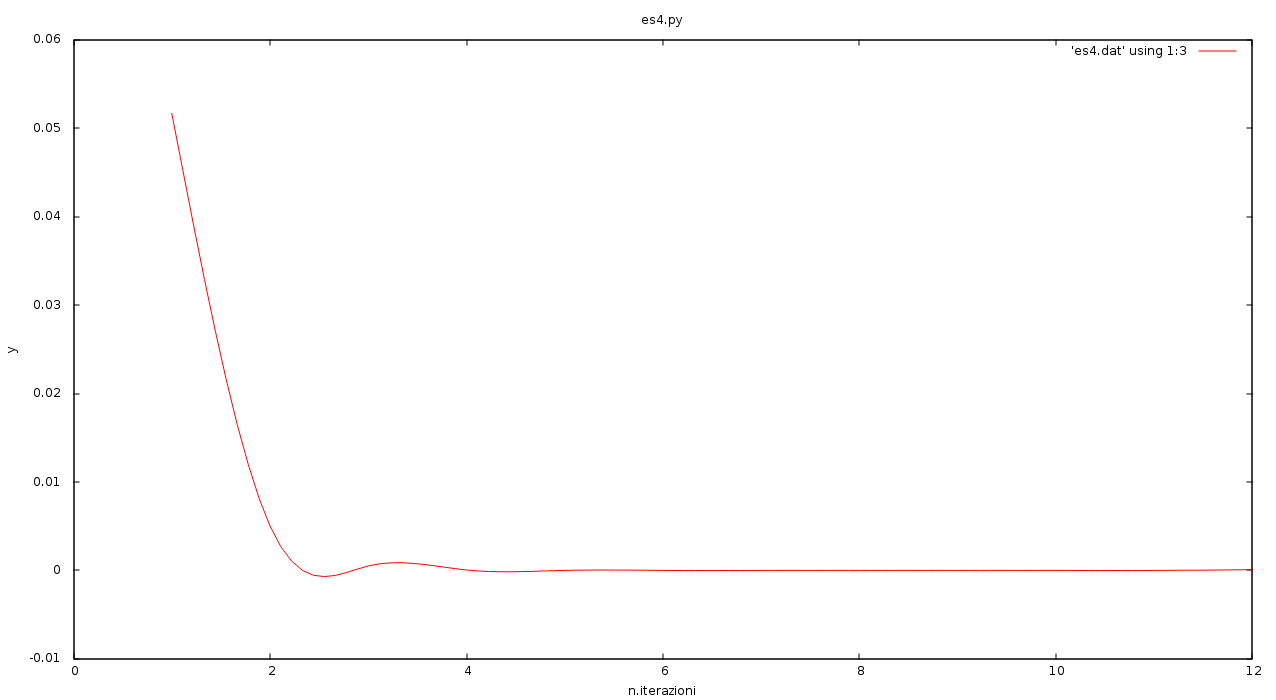
\includegraphics[scale=0.4]{cap_1/es4/es4.png}
